\chapter{Simulações}
\label{chap:Simulacoes}

As simulações\footnote{Todos os arquivos para simulações e a implementação deste trabalho se encontram em um repositório do \emph{GitHub}. Para visualizar as simulações realizadas neste trabalho, acesse o link: https://github.com/MarianaAthayde/tcc/tree/master/Vídeos/Simulações.} realizadas neste trabalho, consideram o robô como um elemento pontual, conforme descrito nas equações \ref{eq:posiçãox}, \ref{eq:posiçãoy} e \ref{eq:posiçãotheta} e foram realizadas com intuito de se observar a viabilidade de implementação da estratégia de controle. 

Essas implementações desconsideram não só o robô como um elemento não-pontual, mas também, desconsideram problemas como: saturação do motor, derrapagem das rodas, falhas de comunicação e imprecisão de leitura dos \emph{encoders}. 

\section{Simulações do Primeiro Problema}
\label{sec:SimulacaoP1}

Primeiramente, foi realizado a simulação da primeira estratégia de abordagem do primeiro problema, em que tem-se uma frota de \emph{N} robôs separados entre si no eixo $y$ e com uma posição randômica no eixo $x$, todos dispostos na mesma direção e sentido. A primeira estratégia elimina os problemas de colisão, visto que os robôs começam separados, no mesmo sentido e como são impossibilitados a imprimir uma velocidade angular pela estratégia adotada, seguem em linha reta com velocidade linear negativa ou positiva. Além disso, ela leva em consideração a rede de comunicação, utilizando-se a \autoref{eq:velP1}. 

Serão feitas simulações com duas redes, a primeira será uma rede centralizada com 4 robôs, tal qual é possível implementar com a plataforma \emph{Lego Mindstorms\textregistered}. A segunda, será uma rede descentralizada com cinco robôs, tal como a rede ilustrada na \autoref{fig:rededistr}. Como mostrado nas figuras \ref{fig:sP1Cent} e \ref{fig:sP1Desc}, essa é uma estratégia viável quando considerando o robô como um elemento pontual.

\begin{figure}[!htb]
	\centering
	\begin{subfigure}{.5\textwidth}
		\centering
		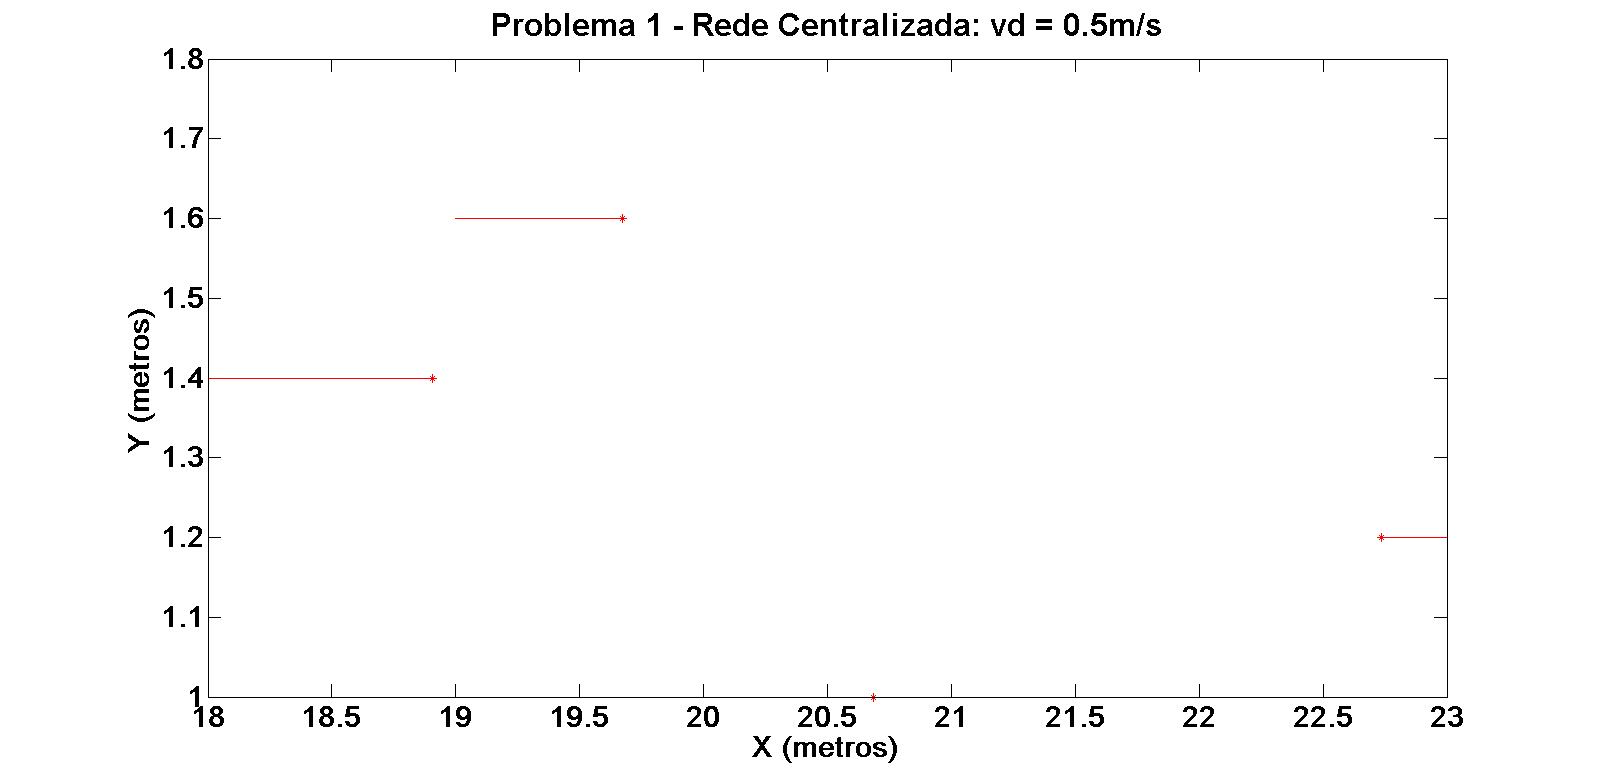
\includegraphics[width=.9\linewidth]{./04-figuras/Simulacoes/Problema1-Abordagem1/P1_A1_Centr_Inicio}
		\caption{Sistema com Rede Centralizada - Antes do alinhamento dos robôs}
		\label{fig:P1CIni}
	\end{subfigure}%
	\begin{subfigure}{.5\textwidth}
		\centering
		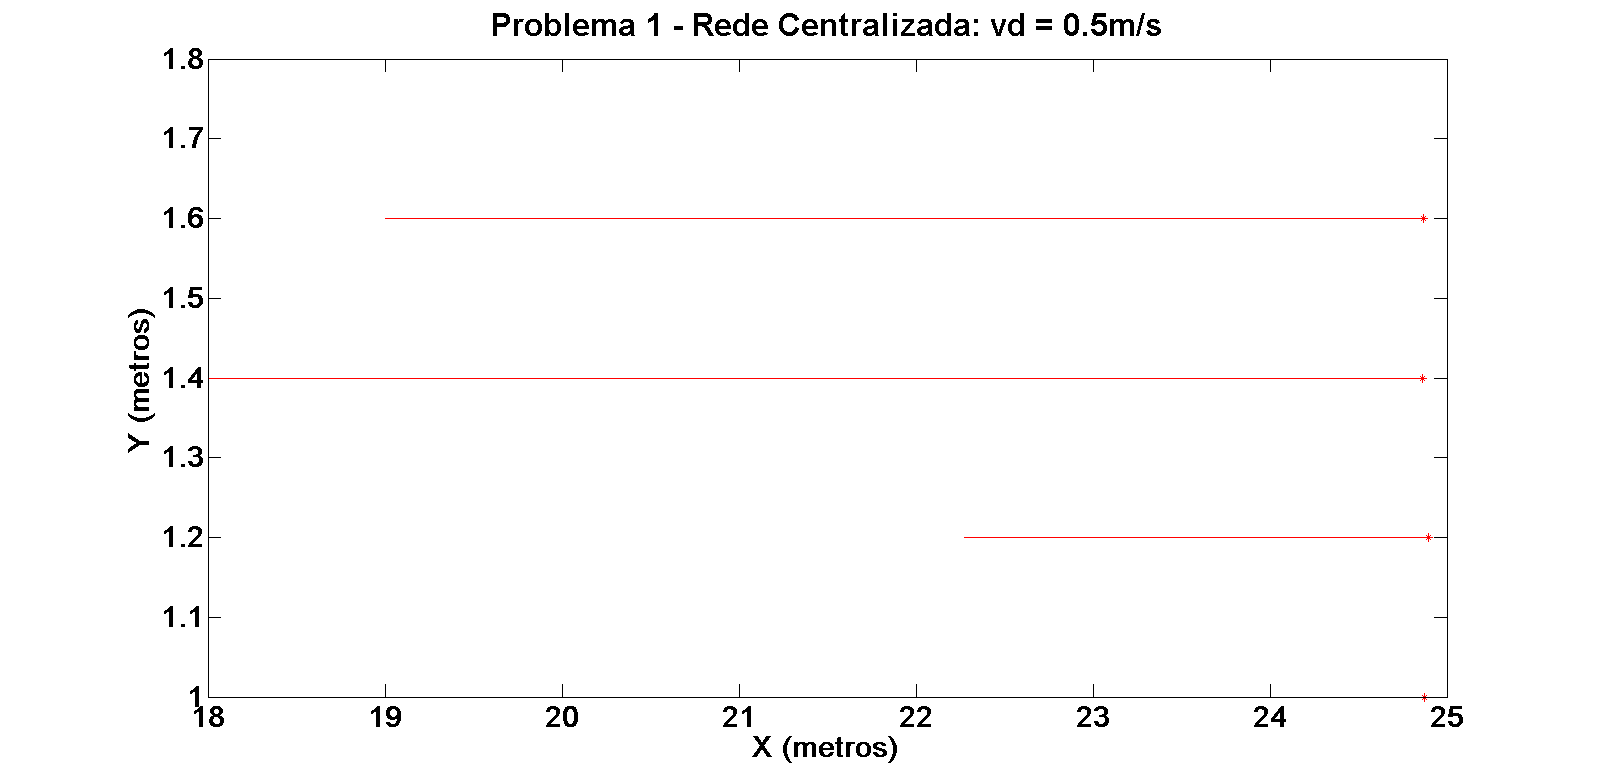
\includegraphics[width=.9\linewidth]{./04-figuras/Simulacoes/Problema1-Abordagem1/P1_A1_Centr_Fim}
		\caption{Sistema com Rede Centralizada - Depois do alinhamento dos robôs}
		\label{fig:P1CFim}
	\end{subfigure}
	\caption{Problema 1 - Primeira Abordagem com Rede Centralizada}
	\label{fig:sP1Cent}
\end{figure}

\begin{figure}[!htb]
	\centering
	\begin{subfigure}{.5\textwidth}
		\centering
		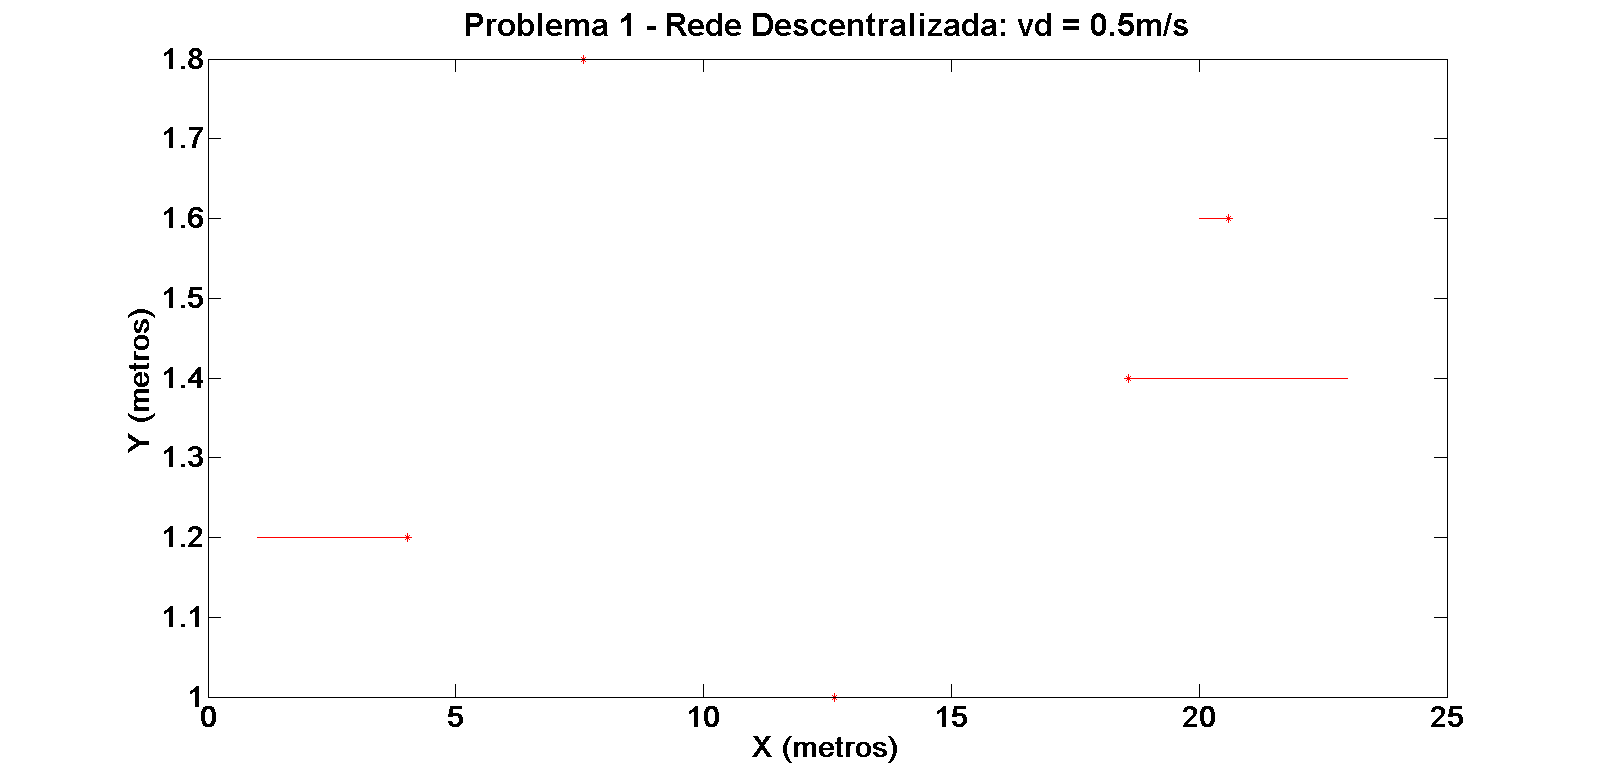
\includegraphics[width=.9\linewidth]{./04-figuras/Simulacoes/Problema1-Abordagem1/P1_A1_Desc_Inicio}
		\caption{Sistema com Rede Descentralizada - Antes do alinhamento dos robôs}
		\label{fig:P1DIni}
	\end{subfigure}%
	\begin{subfigure}{.5\textwidth}
		\centering
		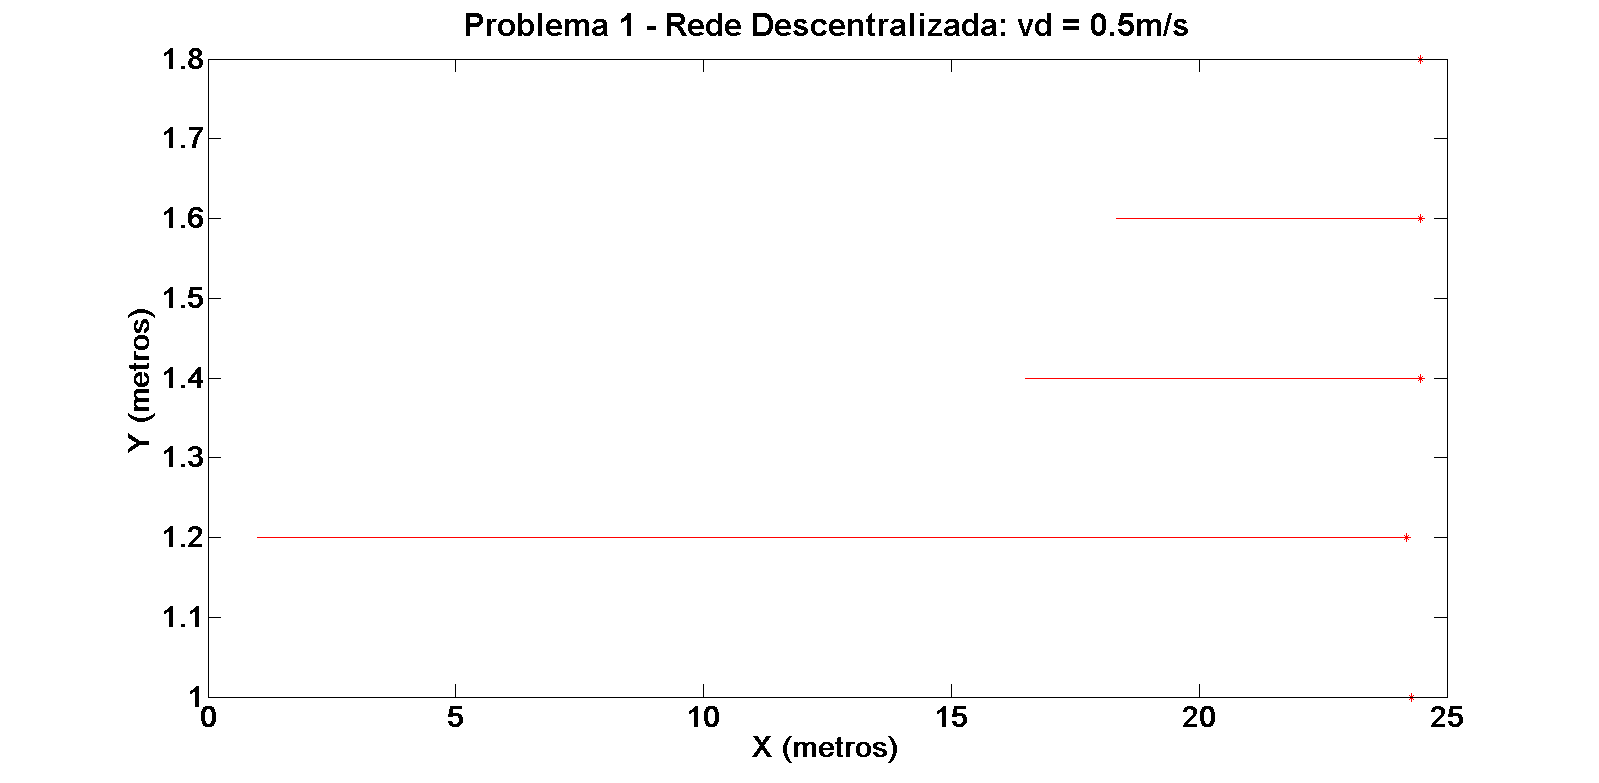
\includegraphics[width=.9\linewidth]{./04-figuras/Simulacoes/Problema1-Abordagem1/P1_A1_Desc_Fim}
		\caption{Sistema com Rede Descentralizada - Depois do alinhamento dos robôs}
		\label{fig:P1DFim}
	\end{subfigure}
	\caption{Problema 1 - Primeira Abordagem com Rede Descentralizada}
	\label{fig:sP1Desc}
\end{figure}

Já a segunda estratégia consiste em encontrar uma reta paralela ao eixo y onde, sua localização no eixo x é a média da posição dos robôs mais distantes entre sí do sistema. Ela foi implementada de modo a permitir que o robô a adquirira uma velocidade angular. Sendo assim ele pode se deslocar em qualquer direção. Essa abordagem faz uso da malha de controle intermediário modelada no \autoref{chap:abordagememdelo} e possui problemas de colisão, já que os robôs podem se deslocar em qualquer direção.

Não foi implementado neste trabalho um tratamento de colisão, foram adotadas algumas medidas para diminuir as colisões no sistema. A primeira medida foi estabelecer uma prioridade na rede que vai do mestre ao último escravo, aquele que possui menor prioridade para ao estar em menos de 20 centímetros de distância de outro robô. A segunda medida foi fazer com que os robôs convirjam um a um para o ponto desejado. Notou-se com essas medidas uma redução no número de colisões ocorridas no sistema. 

Como pode ser visto na \autoref{fig:sP1A2}, essa abordagem também é viável entretanto, apesar de apresentar a vantagem de conceder mais autonomia aos robôs, deixando-os movimentar em qualquer direção, ela acarreta ao sistema problemas de colisão que quando não contornados podem prejudicar o sistema.

\begin{figure}[!htb]
	\centering
	\begin{subfigure}{1.0\textwidth}
		\centering
		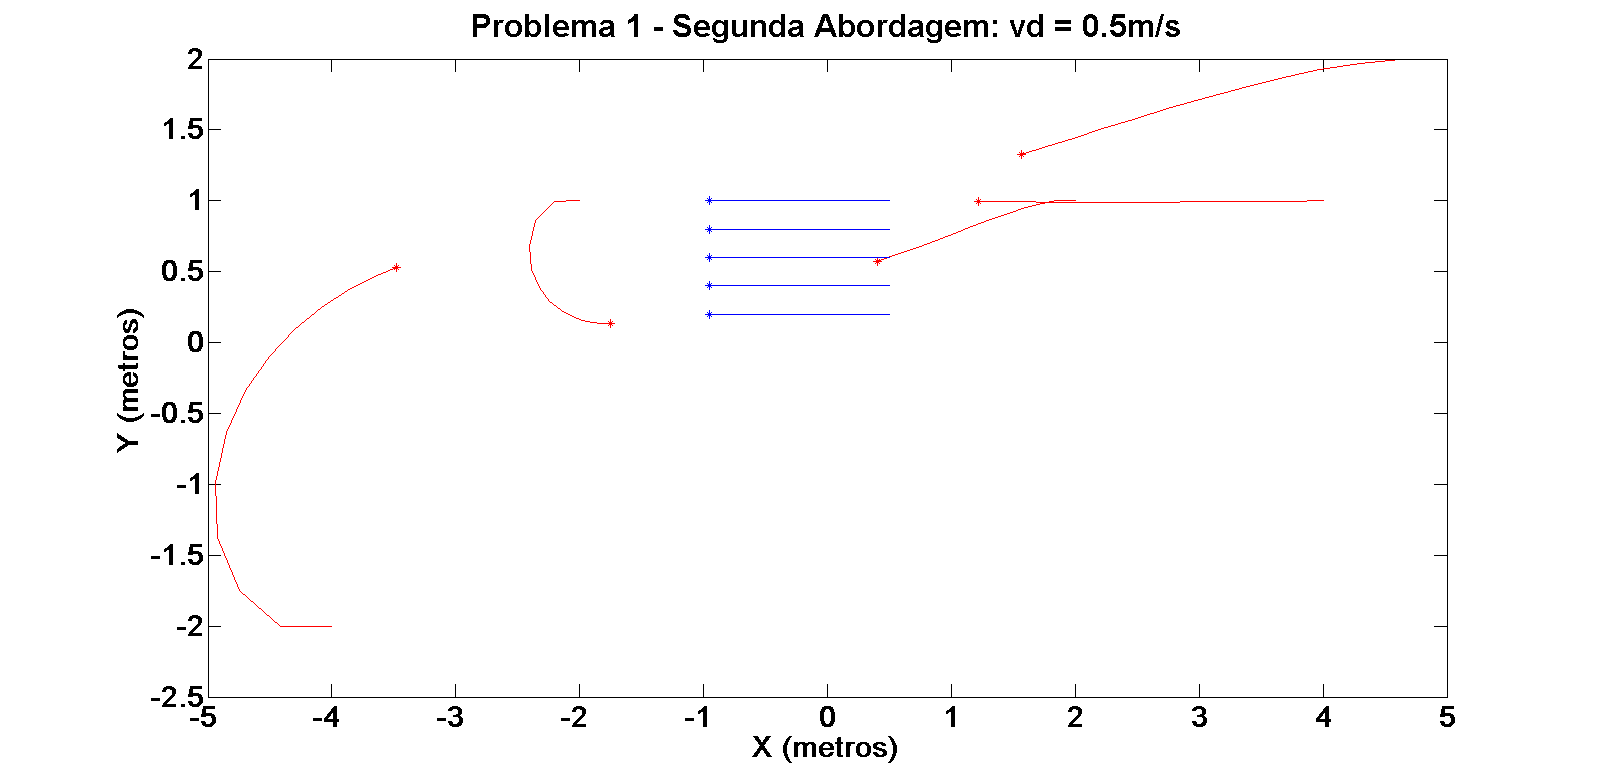
\includegraphics[width=.9\linewidth]{./04-figuras/Simulacoes/Problema1-Abordagem1/P1A2Inicio}
		\caption{Segunda Abordagem - Antes do alinhamento dos robôs}
		\label{fig:P1A2Ini}
	\end{subfigure}
	\begin{subfigure}{1.0\textwidth}
		\centering
		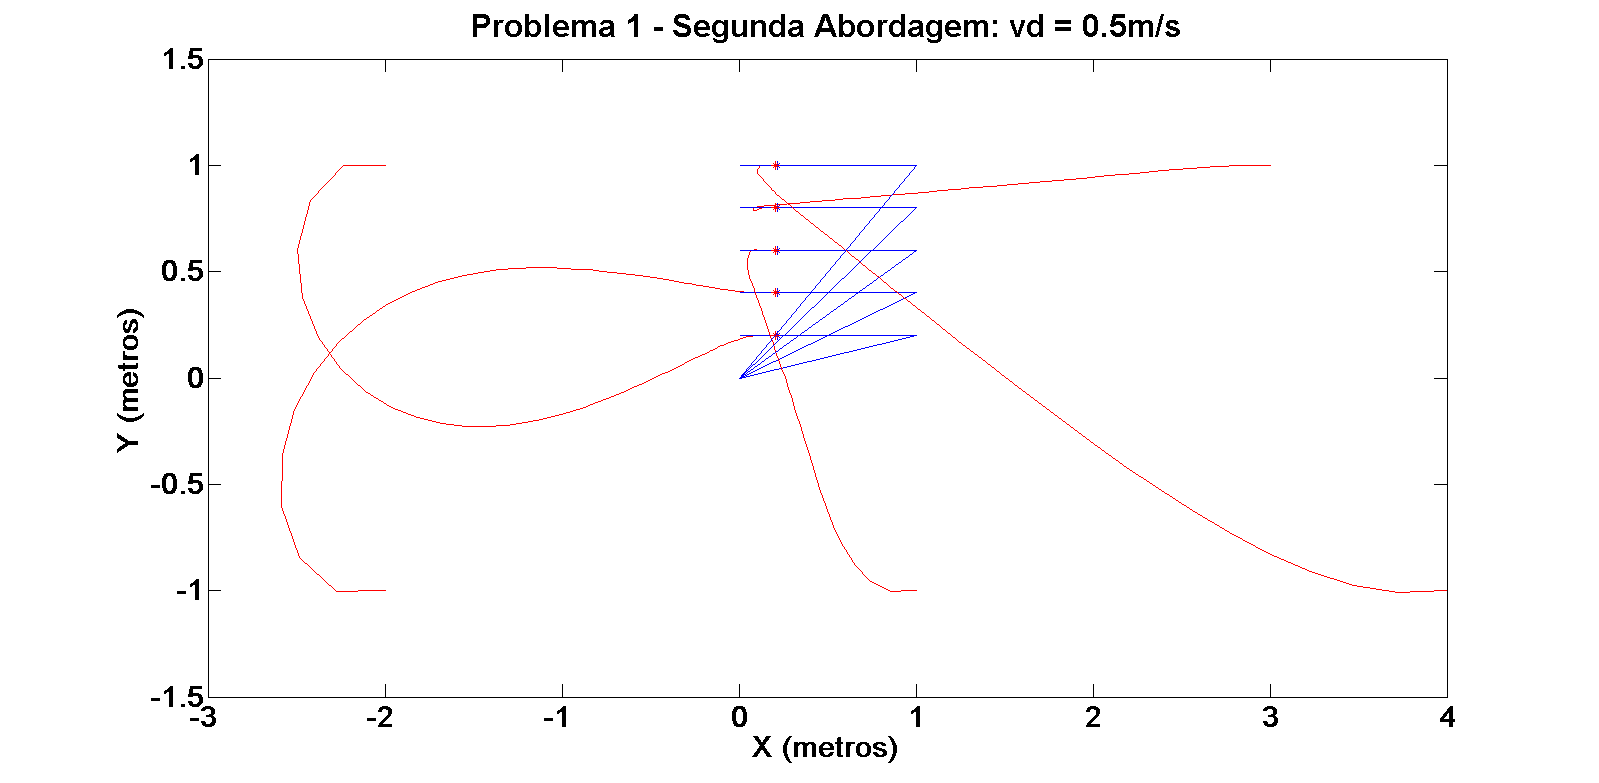
\includegraphics[width=.9\linewidth]{./04-figuras/Simulacoes/Problema1-Abordagem1/P1A2Fim}
		\caption{Segunda Abordagem - Depois do alinhamento dos robôs}
		\label{fig:P1A2Fim}
	\end{subfigure}
	\caption{Problema 1 - Segunda Abordagem}
	\label{fig:sP1A2}
\end{figure}

\section{Simulações do Segundo Problema}
\label{sec:SimulacaoP2}
Como já dito anteriormente neste trabalho, o segundo problema consiste em guiar uma frota de robôs a um determinado alvo e circulá-lo a uma distância \emph{R} e um período \emph{T}. Dito isto, fez-se algumas simulações para validar o modelo matemático e compará-lo ao modelo real. Esta simulação desconsidera um problema enfrentado no mundo real que é a falta de sincronismo entre os relógios dos motores, visto que o tempo corrido em simulação é igual para todos os robôs da frota. 

A primeira simulação realizada desconsidera problemas de colisão e inicia os robôs com posições randômicas, após mil amostras retira-se dois robôs e verifica que os robôs se reorganizam, mantendo a mesma distância entre si. Já nas simulações seguintes tomamos as medidas citadas na \autoref{sec:SimulacaoP1} para evitar que ocorra colisão entre os robôs. Como pode ser visto nas figuras \ref{fig:sP2F}, \ref{fig:sP2C}, as estratégias modeladas são viáveis dentro de um ambiente de simulação pouco realístico. 

\begin{figure}[!htb]
	\centering
	\begin{subfigure}{1.0\textwidth}
		\centering
		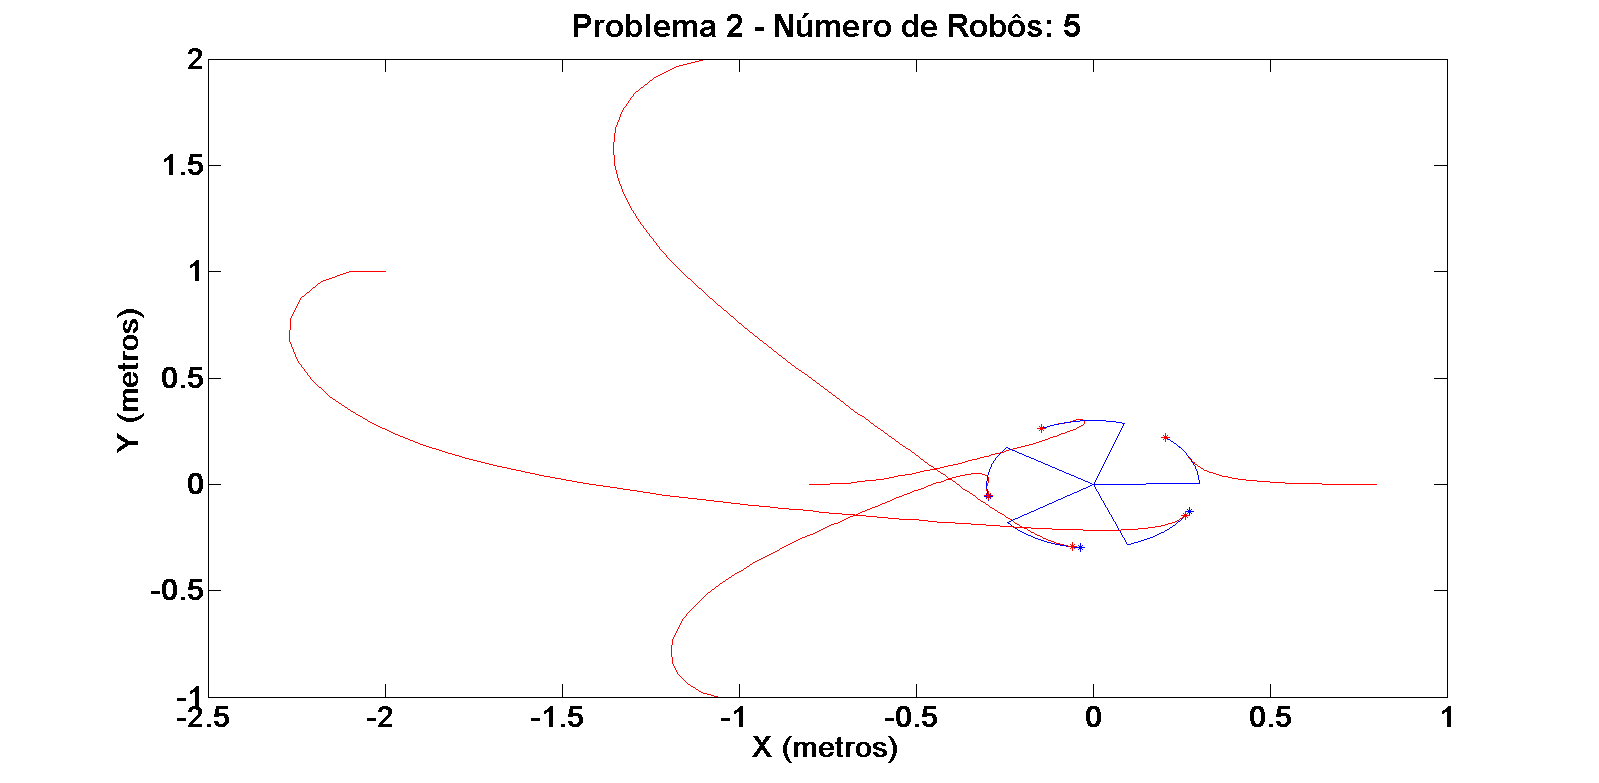
\includegraphics[width=.9\linewidth]{./04-figuras/Simulacoes/Problema2/Falha/P2FalhaInicio}
		\caption{Segundo Problema - Cinco Robôs Alinhados}
		\label{fig:P2SF}
	\end{subfigure}
	\begin{subfigure}{1.0\textwidth}
		\centering
		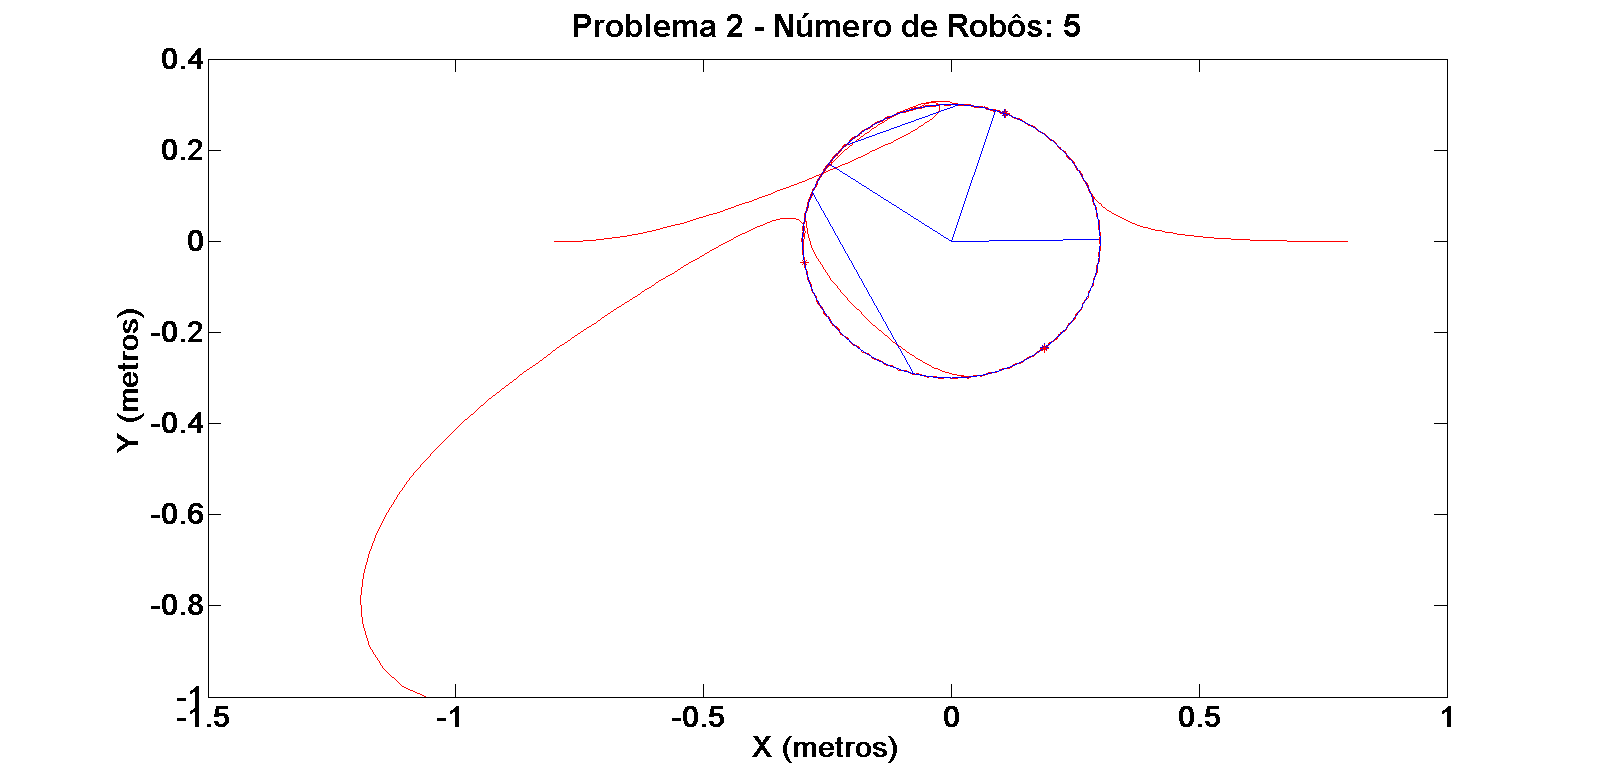
\includegraphics[width=.9\linewidth]{./04-figuras/Simulacoes/Problema2/Falha/P2FalhaFim}
		\caption{Segundo Problema - Falha de 2 Robôs e Reajuste da Formação}
		\label{fig:P2SF2}
	\end{subfigure}
	\caption{Segundo Problema sem Medidas para Evitamento de Colisão}
	\label{fig:sP2F}
\end{figure}

\begin{figure}[!htb]
	\centering
	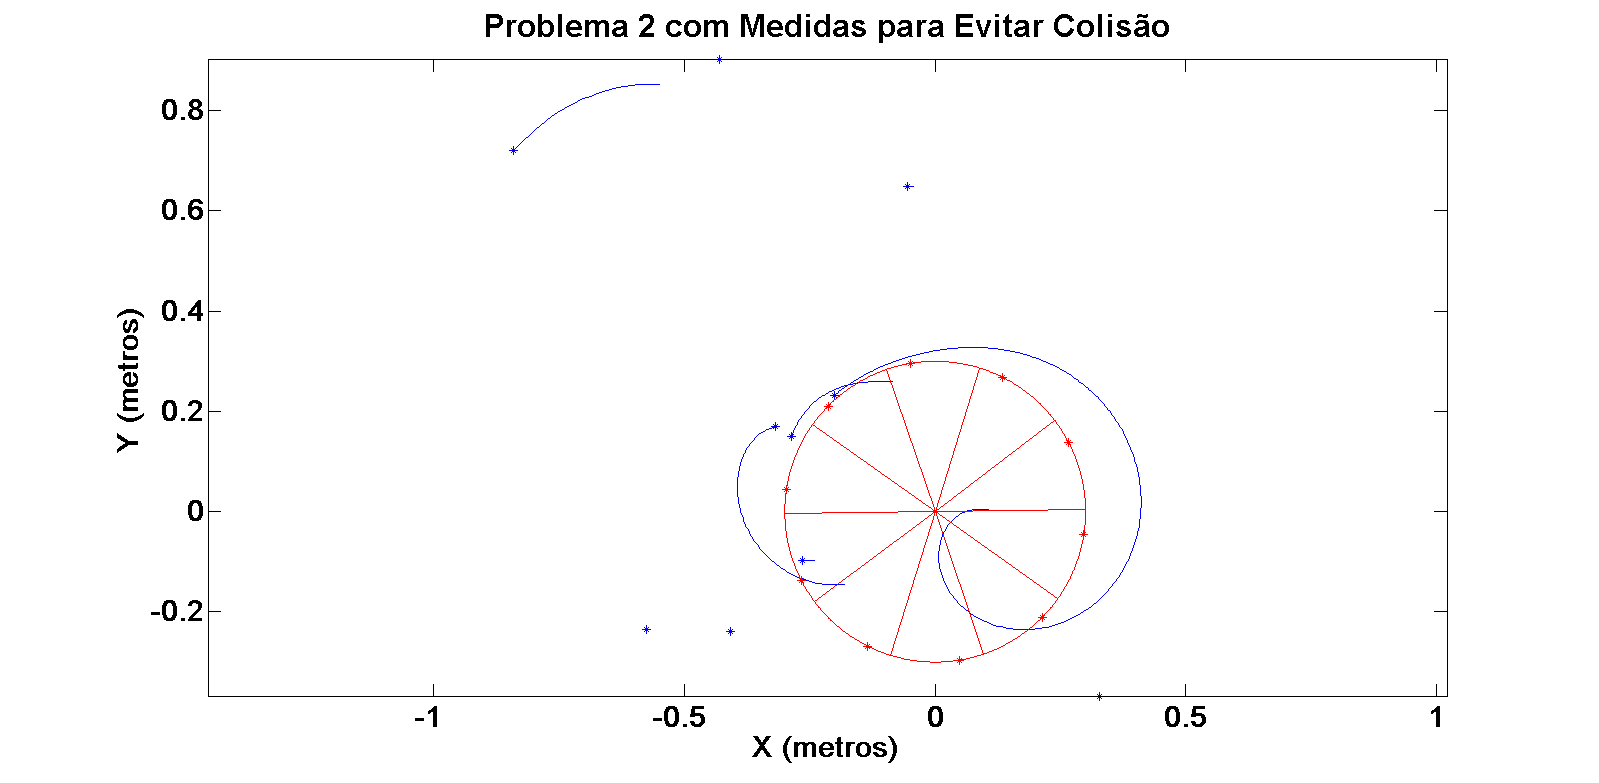
\includegraphics[width=.9\linewidth]{./04-figuras/Simulacoes/Problema2/Colisao/P2_C1}
	\caption{Problema 2: Robôs convergindo um de cada vez, de acordo com a ordem de prioridade}
	\label{fig:P2C}
\end{figure}
